\documentclass[12pt]{article}
\usepackage[margin=1in]{geometry}
\usepackage{graphicx}
\usepackage{amsmath}
\usepackage{amssymb}
\usepackage{booktabs}
\usepackage{float}
\usepackage{subcaption}
\usepackage{hyperref}
\usepackage{listings}
\usepackage{xcolor}

\title{CMPT 742: Assignment 4 Report\\Epipolar Geometry and Fundamental Matrix Estimation}
\author{Yueyang Li 301657120}
\date{\today}

\begin{document}

\maketitle

\section{Introduction}

Epipolar geometry is a fundamental concept in computer vision that describes the geometric relationship between two views of a 3D scene. The fundamental matrix $F$ encodes this relationship and allows us to establish correspondences between points in two images. Given a point $\mathbf{x}_1$ in the first image and its corresponding point $\mathbf{x}_2$ in the second image, they satisfy the epipolar constraint:

\begin{equation}
\mathbf{x}_2^T F \mathbf{x}_1 = 0
\end{equation}

In this assignment, we implement two methods to compute the fundamental matrix: the normalized 8-point algorithm and a robust RANSAC-based approach. We then compare our results with OpenCV's built-in implementation.



\section{Results}

I tested our implementation on three different image pairs. For each pair, I computed three fundamental matrices:
\begin{itemize}
    \item $F_{8pt}$: Using the normalized 8-point algorithm
    \item $F_{RANSAC}$: Using RANSAC with the 8-point algorithm
    \item $F_{OpenCV}$: Using OpenCV's built-in \texttt{findFundamentalMat} function
\end{itemize}

All matrices were normalized by dividing by their $(3,3)$ element for comparison.

\subsection{Test Case 1}

\begin{figure}[H]
    \centering
    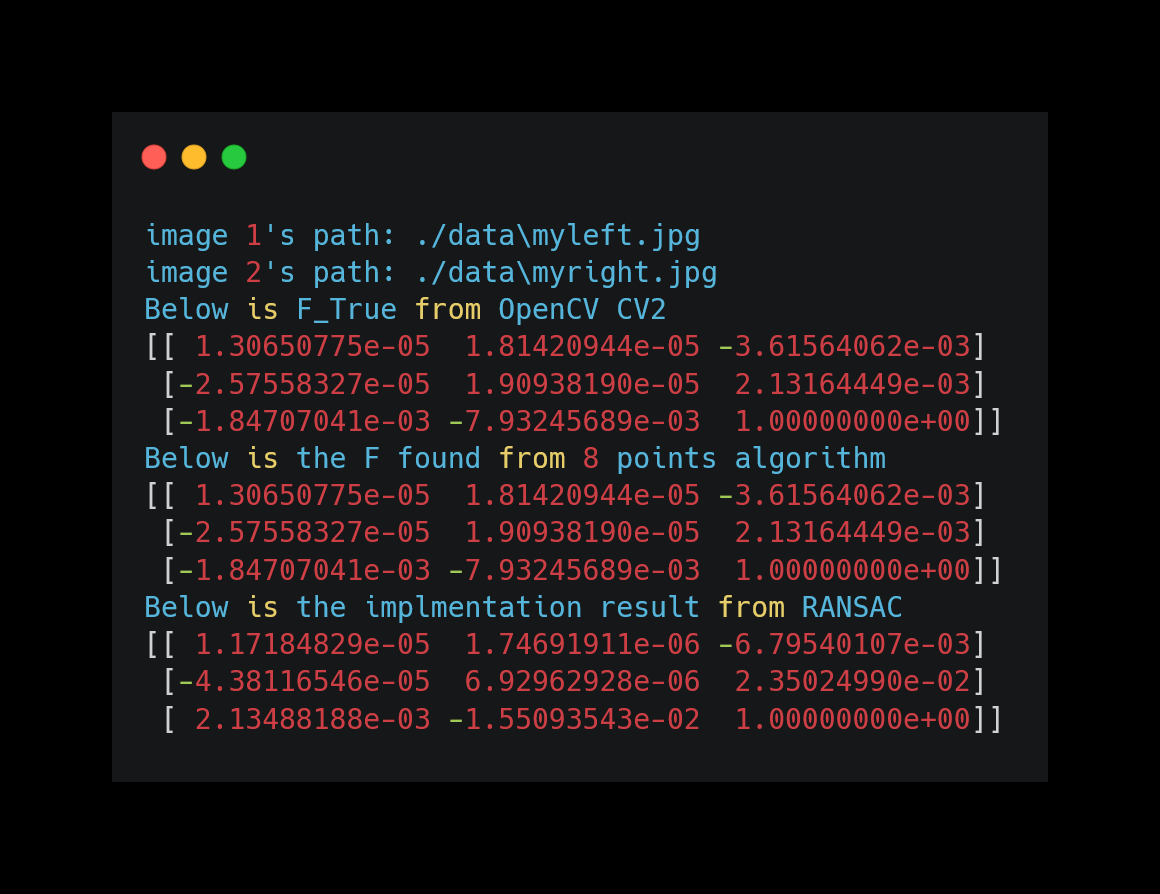
\includegraphics[width=0.95\textwidth]{imgs/comparison_1_parameter.png}
    \caption{Fundamental matrix comparison for Test Case 1. The matrices show excellent agreement between the 8-point algorithm and OpenCV's implementation, while RANSAC provides a robust estimate that filters outliers.}
    \label{fig:comp1_param}
\end{figure}

\begin{figure}[H]
    \centering
    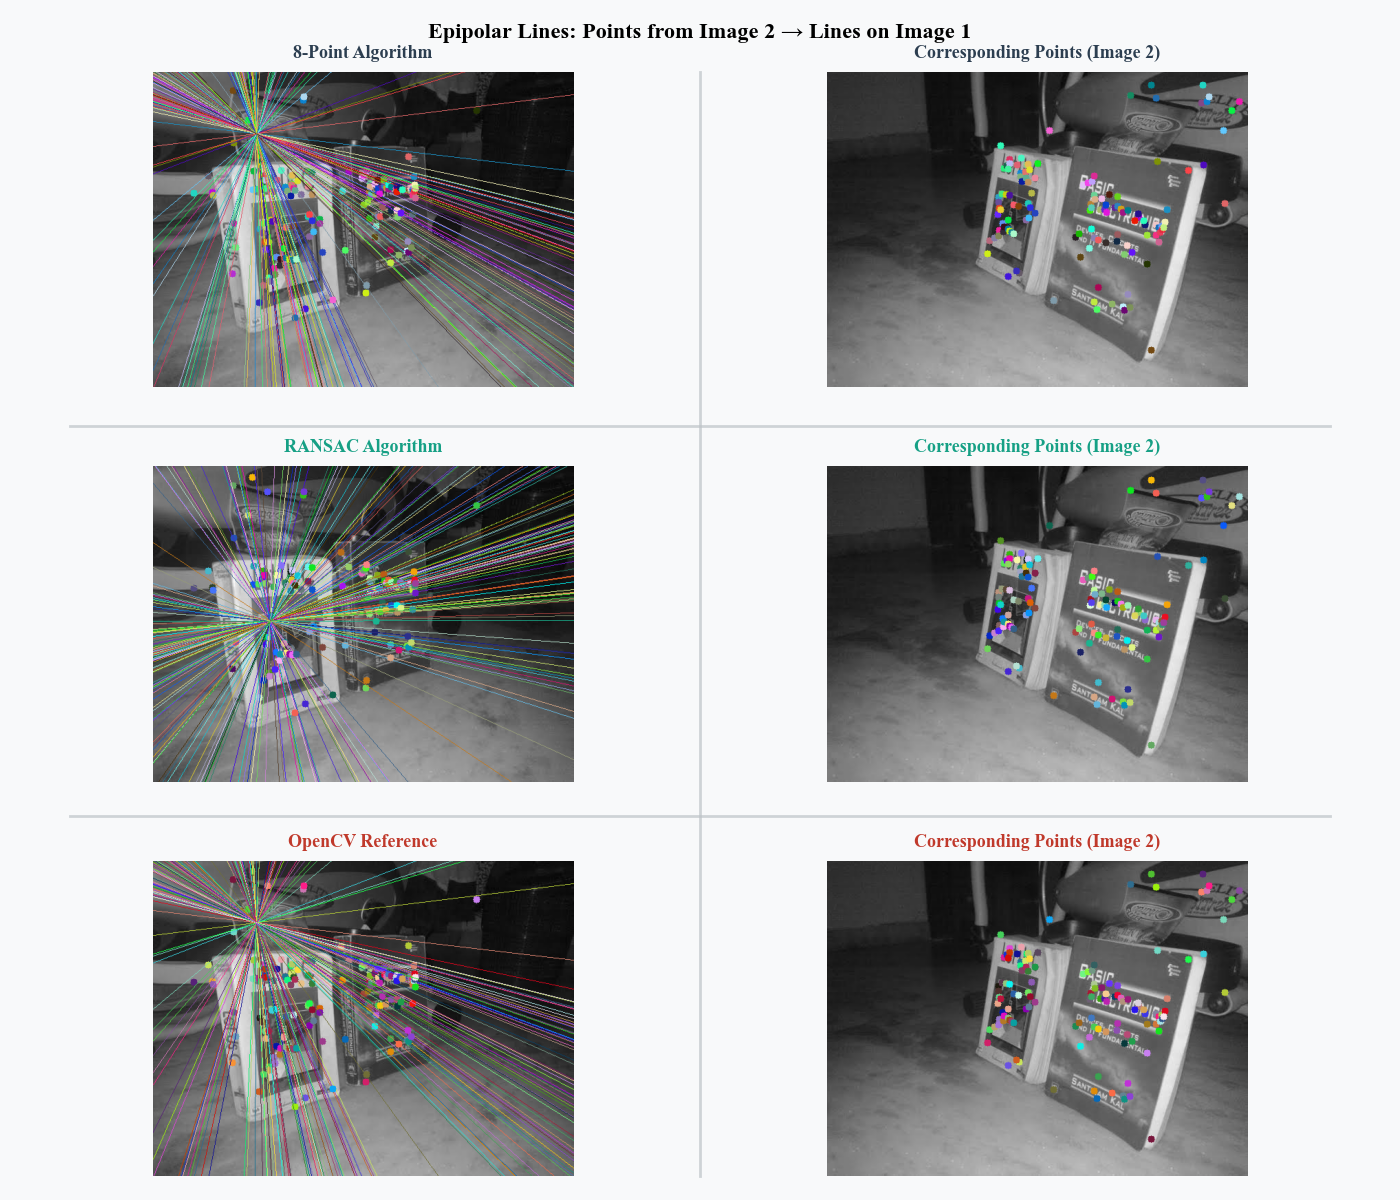
\includegraphics[width=0.95\textwidth]{imgs/comparison_1_left_right.png}
    \caption{Epipolar lines for Test Case 1: Points from Image 2 mapped to epipolar lines on Image 1. Each colored point in Image 2 corresponds to an epipolar line of the same color in Image 1. The quality of the lines indicates the accuracy of the fundamental matrix.}
    \label{fig:comp1_lr}
\end{figure}

\begin{figure}[H]
    \centering
    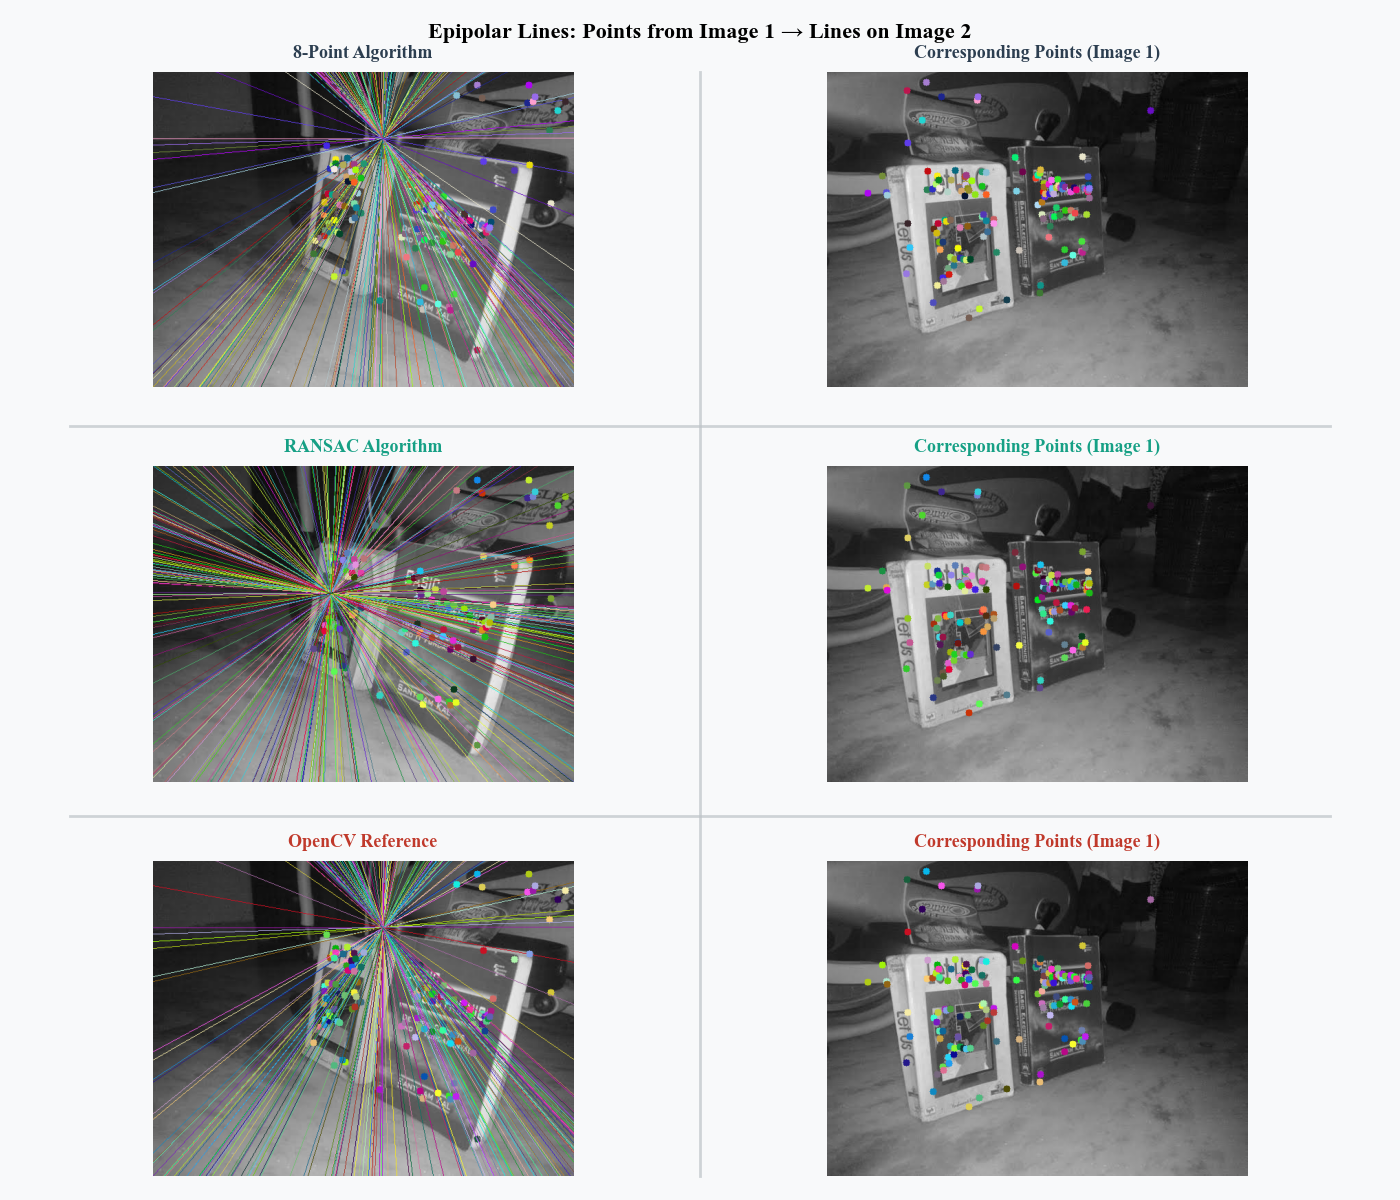
\includegraphics[width=0.95\textwidth]{imgs/comparison_1_right_left.png}
    \caption{Epipolar lines for Test Case 1: Points from Image 1 mapped to epipolar lines on Image 2. This demonstrates the symmetric nature of epipolar geometry.}
    \label{fig:comp1_rl}
\end{figure}

\textbf{Analysis}: For Test Case 1, the 8-point algorithm produces results nearly identical to OpenCV's implementation, confirming the correctness of our normalization and SVD approach. The RANSAC method shows similar epipolar line quality, indicating that the keypoint matches contain relatively few outliers in this case.

\subsection{Test Case 2}

\begin{figure}[H]
    \centering
    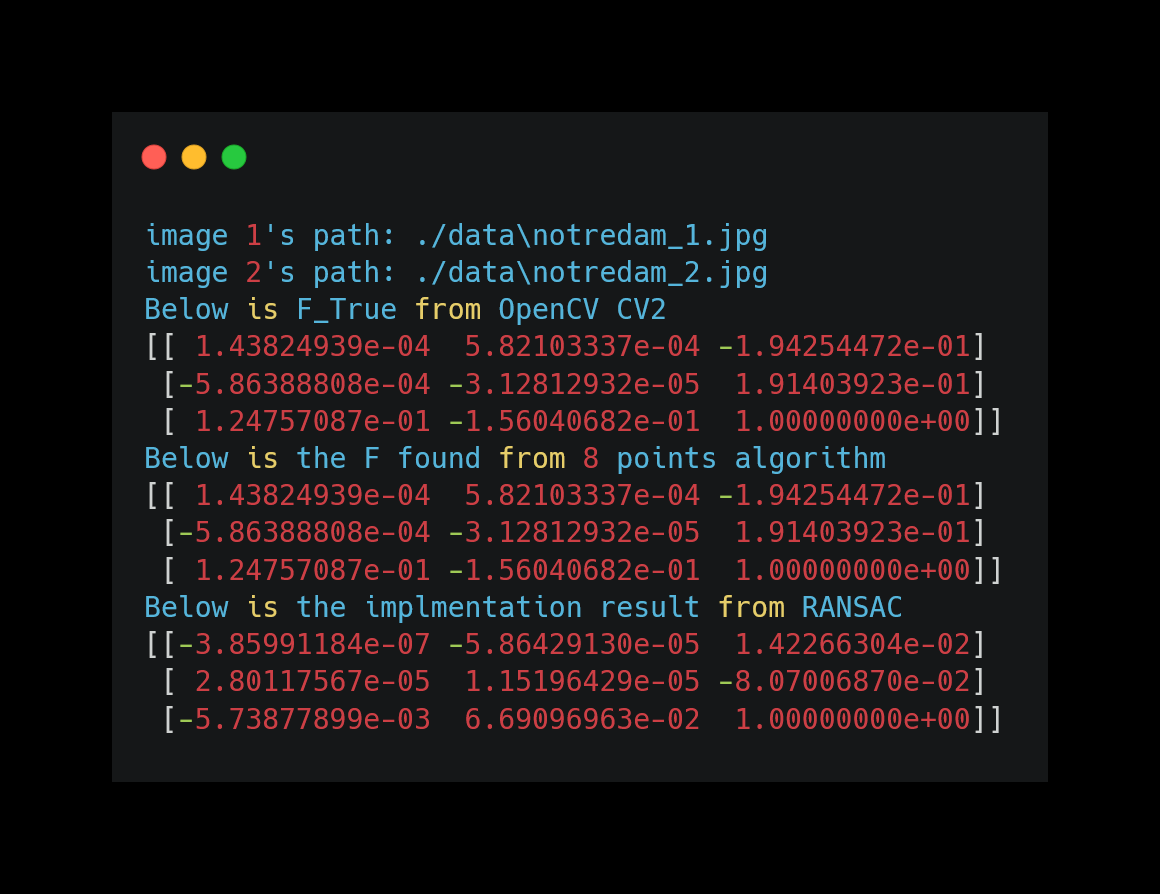
\includegraphics[width=0.95\textwidth]{imgs/comparison_2_parameter.png}
    \caption{Fundamental matrix comparison for Test Case 2. Note the variation in matrix values between different methods, particularly for RANSAC.}
    \label{fig:comp2_param}
\end{figure}

\begin{figure}[H]
    \centering
    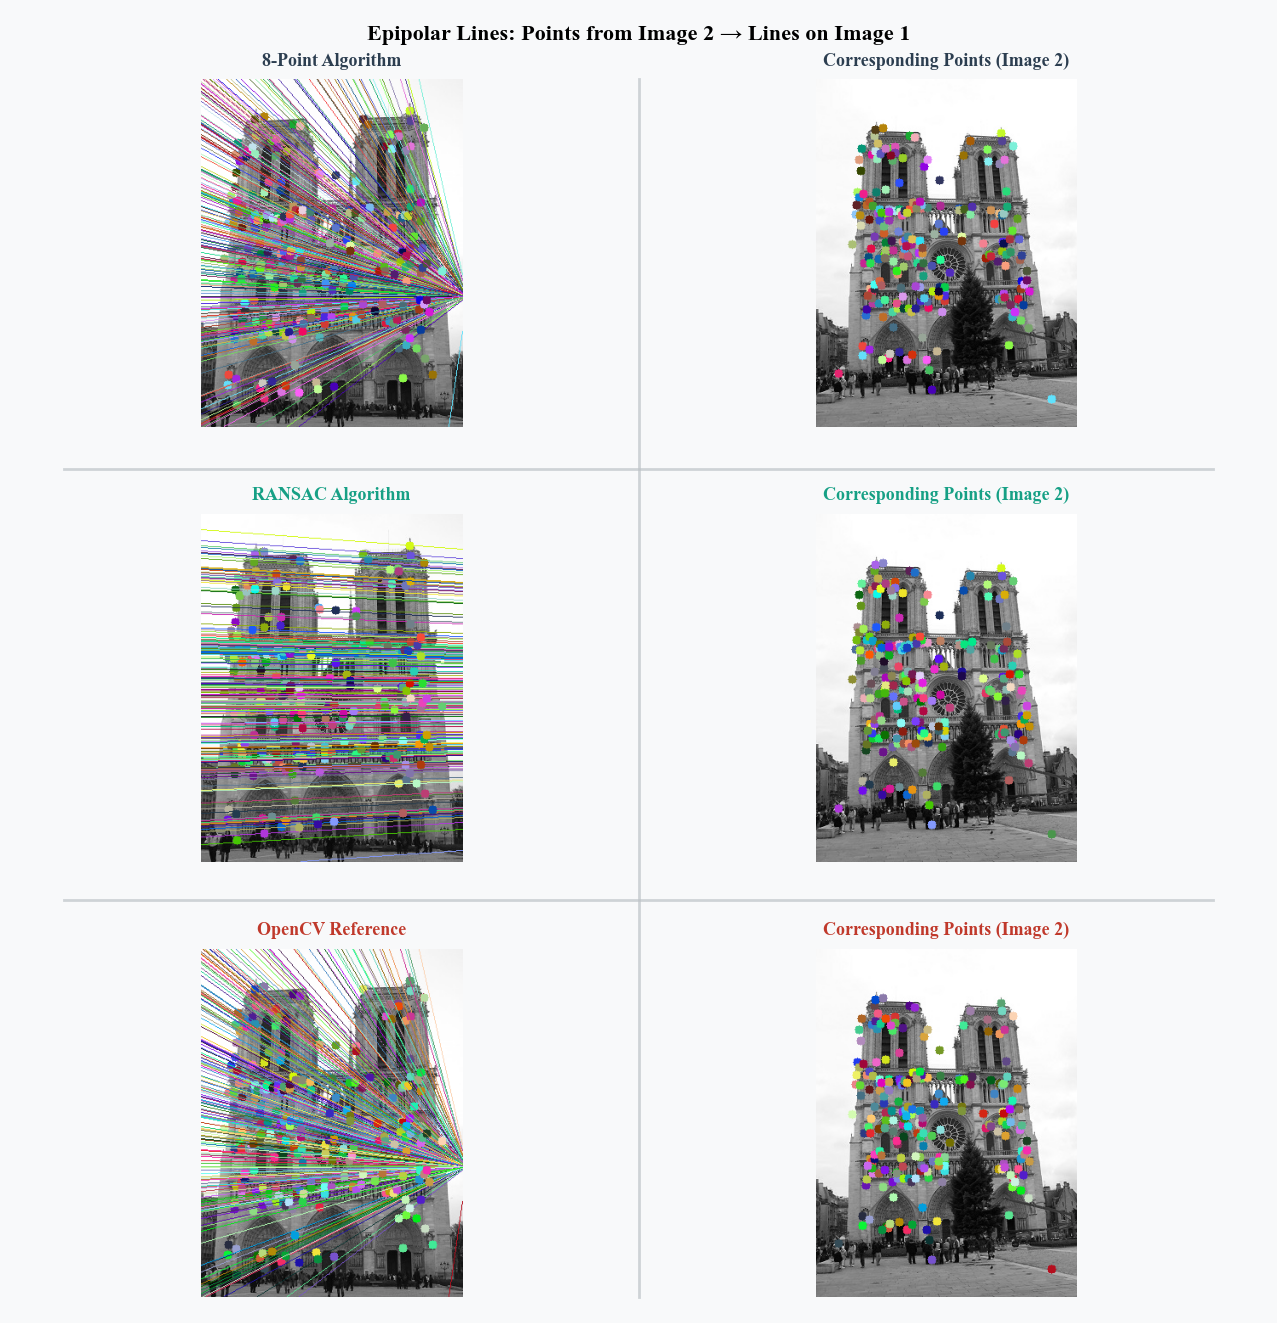
\includegraphics[width=0.95\textwidth]{imgs/comparison_2_left_right.png}
    \caption{Epipolar lines for Test Case 2: Points from Image 2 to lines on Image 1. The RANSAC method shows improved line quality compared to the standard 8-point algorithm, suggesting the presence of outliers.}
    \label{fig:comp2_lr}
\end{figure}

\begin{figure}[H]
    \centering
    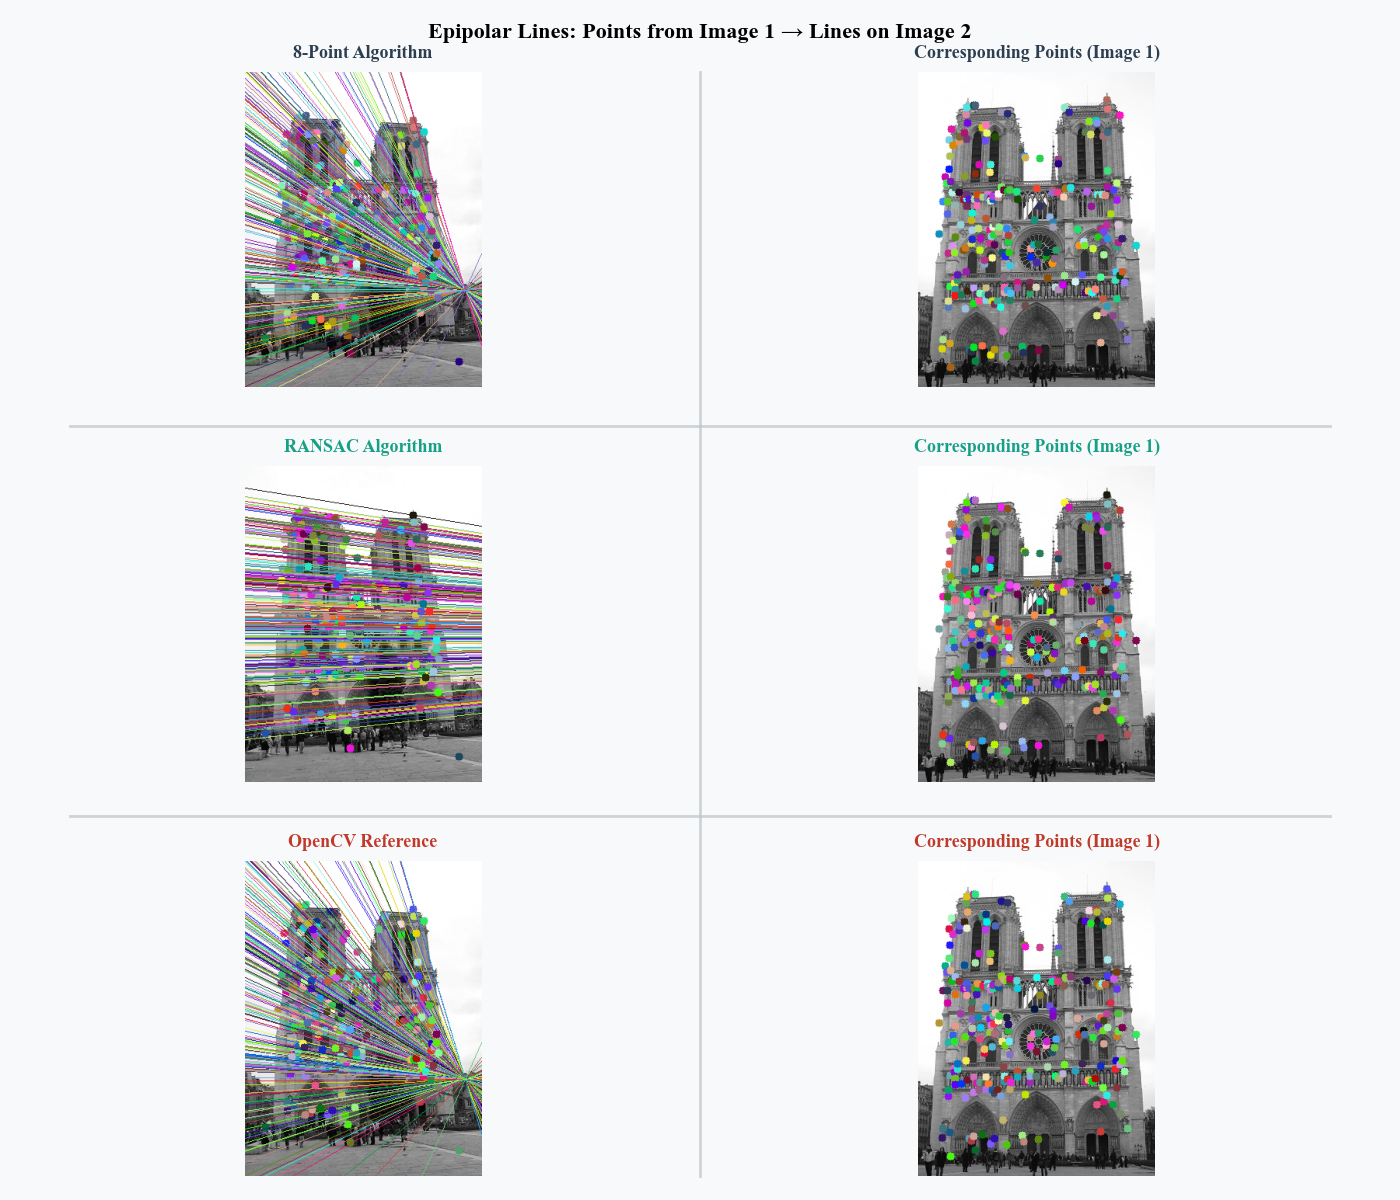
\includegraphics[width=0.95\textwidth]{imgs/comparison_2_right_left.png}
    \caption{Epipolar lines for Test Case 2: Points from Image 1 to lines on Image 2.}
    \label{fig:comp2_rl}
\end{figure}

\textbf{Analysis}: In Test Case 2, we observe greater variation between the three methods. The RANSAC algorithm's fundamental matrix differs more significantly from the 8-point result, suggesting that RANSAC successfully filtered out outlier correspondences. The epipolar lines from RANSAC appear more consistent and better aligned with the corresponding points.

\subsection{Test Case 3}

\begin{figure}[H]
    \centering
    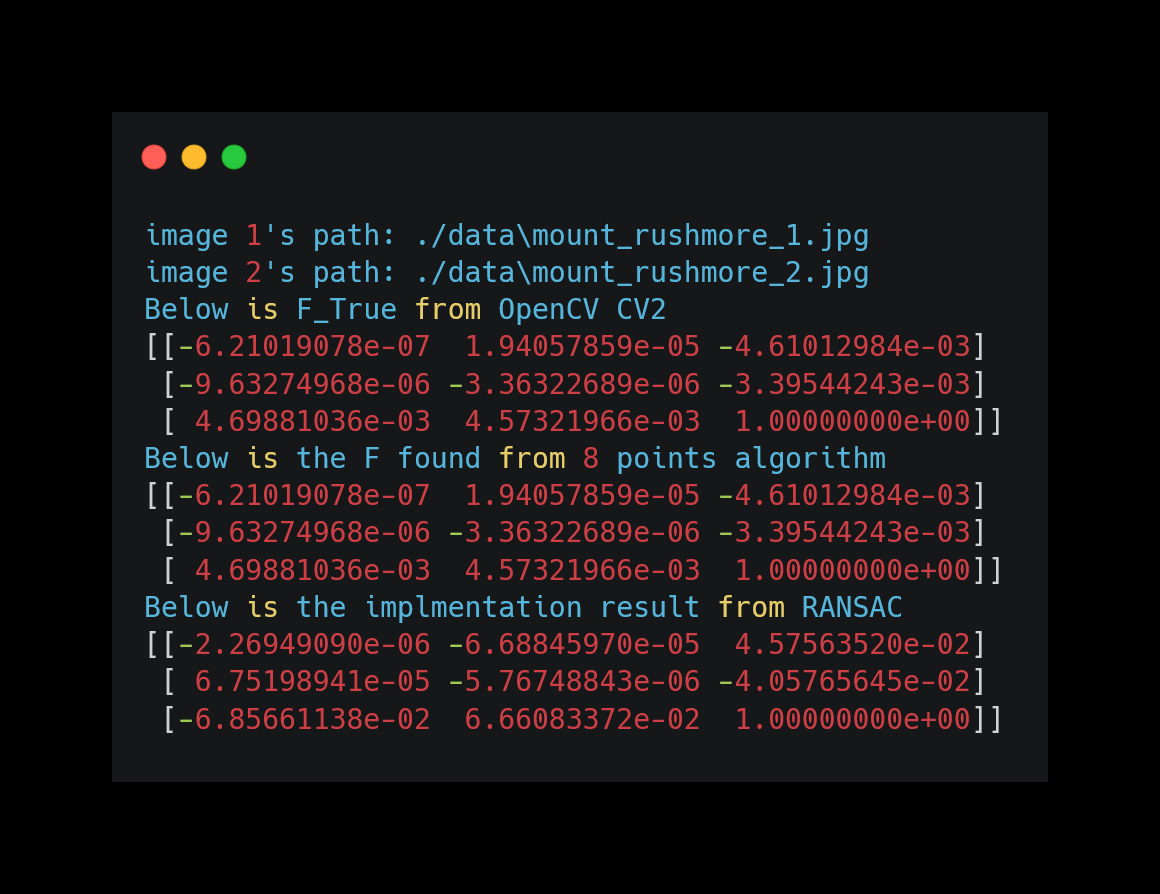
\includegraphics[width=0.95\textwidth]{imgs/comparison_3_parameter.png}
    \caption{Fundamental matrix comparison for Test Case 3. The matrices demonstrate the robustness of RANSAC in challenging scenarios.}
    \label{fig:comp3_param}
\end{figure}

\begin{figure}[H]
    \centering
    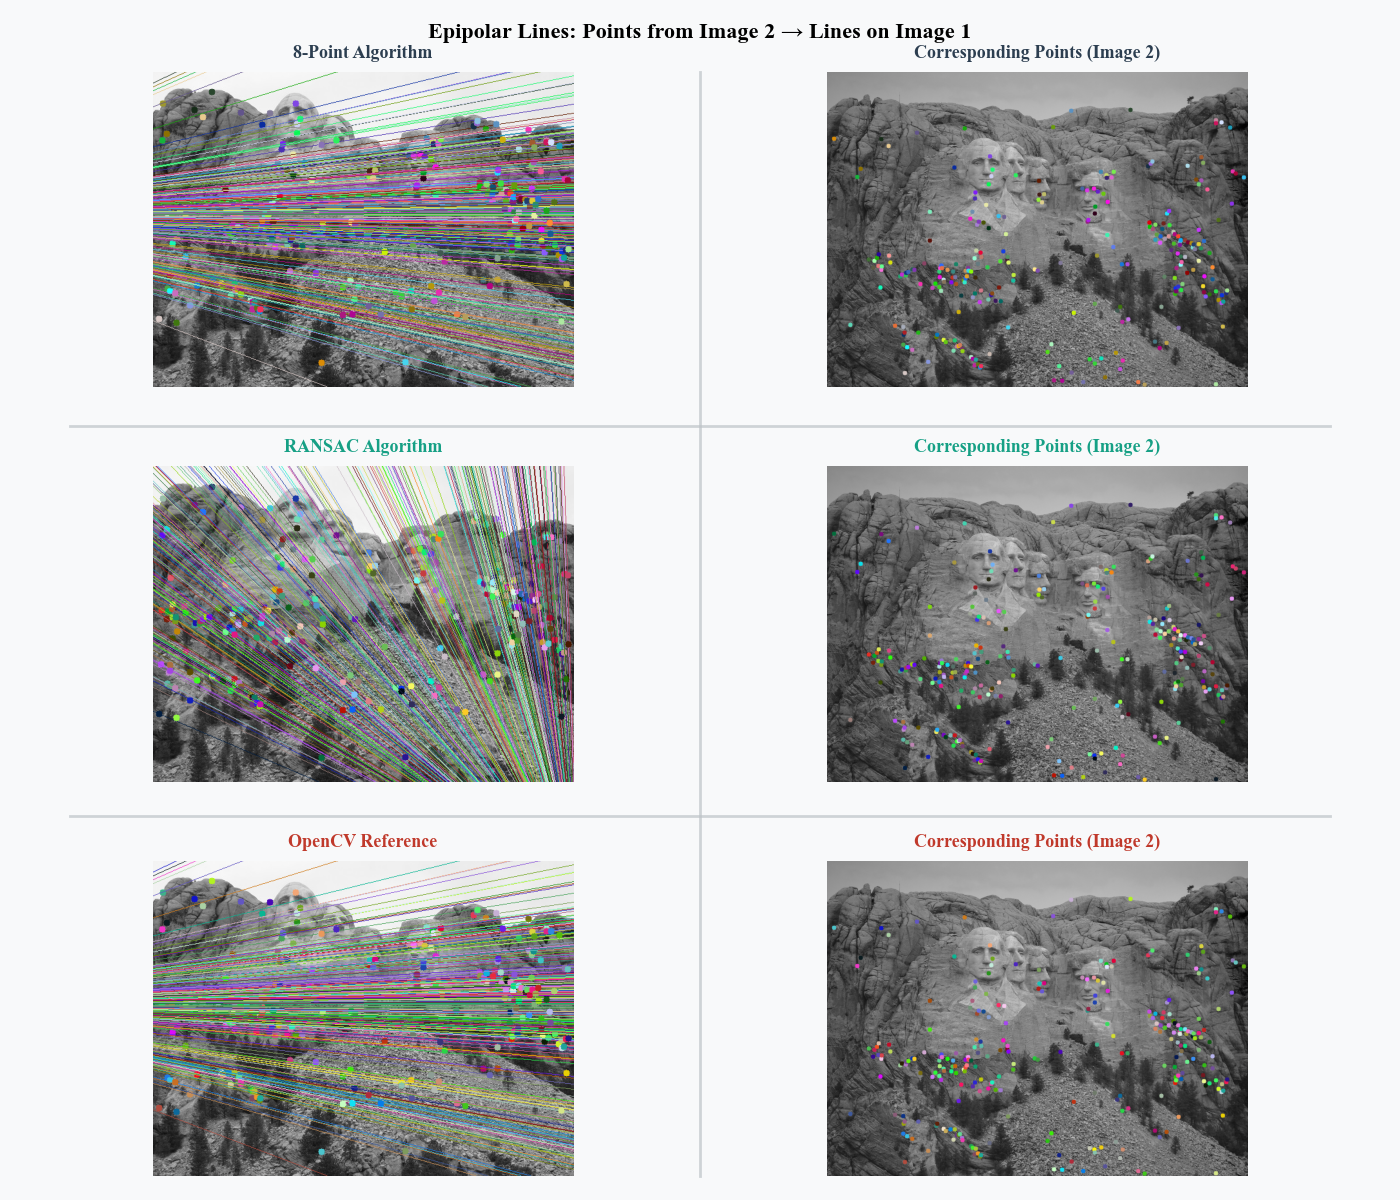
\includegraphics[width=0.95\textwidth]{imgs/comparison_3_left_right.png}
    \caption{Epipolar lines for Test Case 3: Points from Image 2 to lines on Image 1. This test case demonstrates the importance of RANSAC when dealing with noisy correspondences.}
    \label{fig:comp3_lr}
\end{figure}

\begin{figure}[H]
    \centering
    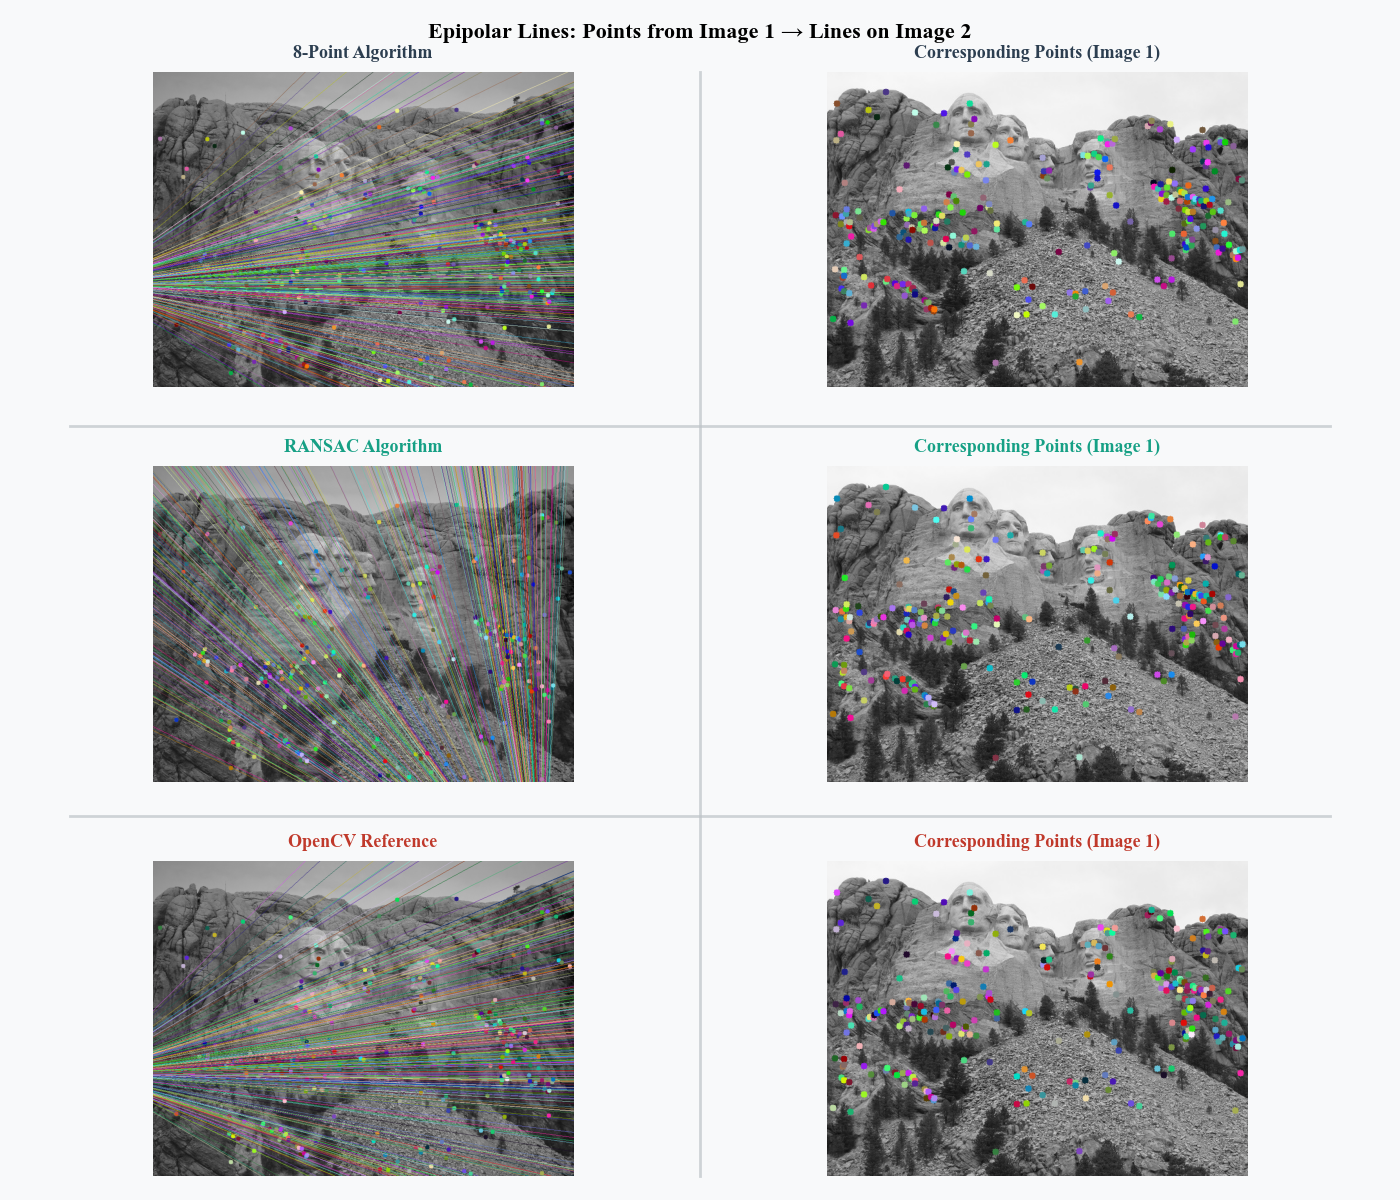
\includegraphics[width=0.95\textwidth]{imgs/comparison_3_right_left.png}
    \caption{Epipolar lines for Test Case 3: Points from Image 1 to lines on Image 2.}
    \label{fig:comp3_rl}
\end{figure}

\textbf{Analysis}: Test Case 3 shows the most significant differences between methods. The RANSAC implementation provides noticeably cleaner epipolar geometry, with lines that pass more accurately through or very close to the corresponding points. This demonstrates RANSAC's effectiveness in handling outliers from imperfect keypoint detection and matching.


\end{document}